% Completed solutions for Homework 5.
\documentclass[11pt,addpoints,answers]{exam}

\newcommand{\hwnum}{5}
\newcommand{\duedate}{October 7}

\RequirePackage{microtype}
\RequirePackage{mathtools}
\RequirePackage{amsthm}
\RequirePackage{amssymb}
\RequirePackage{xspace}
\RequirePackage[shortlabels]{enumitem}
\RequirePackage{xcolor}
\RequirePackage{hyperref}
\RequirePackage[capitalize,nameinlink,noabbrev]{cleveref} % must load after hyperref
\usepackage{fvextra} % To use Verbatim
\usepackage{diagbox} % For diagbox
\RequirePackage[boxed]{algorithm}
\RequirePackage[noend]{algpseudocode}
\RequirePackage{tikz}
\usetikzlibrary{arrows,automata,positioning}

\hypersetup{breaklinks=true,
    colorlinks=true,
    linkcolor=blue,
    filecolor=blue,
    citecolor=blue,
    urlcolor=blue}

\algrenewcommand{\algorithmiccomment}[1]{\texttt{//} #1}
\algrenewcommand\algorithmicrequire{\textbf{Input:}}
\algrenewcommand\algorithmicensure{\textbf{Output:}}


% allow cleveref to label and reference enumerables defined in the exam class.
% these automatically define corresponding \Crefname as well.

% https://tex.stackexchange.com/questions/126020/cleveref-doesnt-use-correct-capitalized-name-if-used-with-amsthm
\makeatletter
\if@cref@capitalise
\crefname{question}{Question}{Questions}
\Crefname{partno}{Part}{Parts}
\crefname{subpart}{Subpart}{Subparts)}
\crefname{subsubpart}{Subsubpart}{Subsubparts}
\else
\crefname{question}{question}{questions}
\crefname{partno}{part}{parts}
\crefname{subpart}{subpart}{subparts}
\crefname{subsubpart}{subsubpart}{subsubparts}
\fi
\makeatother

% numeric sets in "blackboard" font

\newcommand{\N}{\mathbb{N}}
\newcommand{\Z}{\mathbb{Z}}
\newcommand{\R}{\mathbb{R}}
\newcommand{\Q}{\mathbb{Q}}
\newcommand{\C}{\mathbb{C}}
\newcommand{\Prop}{\mathbb{P}}

% paired delimiters

\DeclarePairedDelimiter\abs{\lvert}{\rvert}
\DeclarePairedDelimiter\length{\lVert}{\rVert}
\DeclarePairedDelimiter\norm{\lVert}{\rVert}
\DeclarePairedDelimiter\parens{(}{)}
\DeclarePairedDelimiter\tuple{(}{)}
\DeclarePairedDelimiter\brackets{[}{]}
\DeclarePairedDelimiter\floor{\lfloor}{\rfloor}
\DeclarePairedDelimiter\ceil{\lceil}{\rceil}
\DeclarePairedDelimiter\round{\lfloor}{\rceil}
\DeclarePairedDelimiter\set{\{}{\}}
\DeclarePairedDelimiter\inner{\langle}{\rangle}

\newcommand{\bit}{\set{0,1}}

% asymptotics

\DeclareMathOperator{\Otil}{\tilde{O}}
\DeclareMathOperator{\poly}{poly}
\DeclareMathOperator{\polylog}{polylog}
\DeclareMathOperator{\negl}{negl}

% algorithms

\newcommand{\algo}[1]{\textsc{#1}}

\newcommand{\memo}{\text{memo}}
\newcommand{\tabl}{\text{table}}
\newcommand{\backtrack}{\text{backtrack}}

\newcommand{\ALG}{\text{ALG}}
\newcommand{\OPT}{\text{OPT}}
\newcommand{\weight}{\text{weight}}
\newcommand{\val}{\text{value}}

% computability

% named language
\newcommand{\lang}[1]{L_{\text{#1}}}
% computational problem
\newcommand{\cproblem}[1]{\ensuremath{\text{#1}}\xspace}
% class of languages
\newcommand{\class}[1]{\ensuremath{\mathsf{#1}}\xspace}

\newcommand{\qst}{q_{\text{start}}}
\newcommand{\qacc}{q_{\text{acc}}}
\newcommand{\qrej}{q_{\text{rej}}}

\newcommand{\Lbarber}{\lang{BARBER}}
\newcommand{\atm}{\lang{ACC}}
\newcommand{\htm}{\lang{HALT}}
\newcommand{\ehtm}{\lang{$\varepsilon$-HALT}}
\newcommand{\eqtm}{\lang{EQ}}
\newcommand{\etm}{\lang{$\emptyset$}}
\newcommand{\epstm}{\lang{$\set{\varepsilon}$}}
\newcommand{\Lprop}{\lang{$\Prop$}}
\newcommand{\LSigmastar}{\lang{$\Sigma^*$}}

% complexity

\newcommand{\yes}{\ensuremath{\text{YES}}}
\newcommand{\no}{\ensuremath{\text{NO}}}

\newcommand{\DTIME}{\class{DTIME}}
\renewcommand{\P}{\class{P}}
\newcommand{\NP}{\class{NP}}
\newcommand{\NPH}{\class{NPH}}
\newcommand{\NPC}{\class{NPC}}
\newcommand{\coNP}{\class{coNP}}

\newcommand{\MAZE}{\cproblem{MAZE}}
\newcommand{\PALINDROME}{\cproblem{PALINDROME}}
\newcommand{\TSP}{\cproblem{TSP}}
\newcommand{\SAT}{\cproblem{SAT}}
\newcommand{\CSAT}{\cproblem{CSAT}}
\newcommand{\TSAT}{\cproblem{3SAT}}
\newcommand{\VC}{\cproblem{VERTEX-COVER}}
\newcommand{\DS}{\cproblem{DOMINATING-SET}}
\newcommand{\SC}{\cproblem{SET-COVER}}
\newcommand{\HC}{\cproblem{HAMCYCLE}}
\newcommand{\HP}{\cproblem{HAMPATH}}
\newcommand{\AHP}{\cproblem{ANYHAMPATH}}
\newcommand{\IS}{\cproblem{IS}}
\newcommand{\CLIQUE}{\cproblem{CLIQUE}}
\newcommand{\SSUM}{\cproblem{SUBSET-SUM}}
\newcommand{\KNAPSACK}{\cproblem{KNAPSACK}}
\newcommand{\MAXCUT}{\cproblem{MAX-CUT}}

% randomness

\DeclareMathOperator*{\Var}{Var}
\DeclareMathOperator*{\Ex}{\mathbb{E}}

\newcommand{\RP}{\class{RP}}
\newcommand{\coRP}{\class{coRP}}
\newcommand{\BPP}{\class{BPP}}
\newcommand{\ZPP}{\class{ZPP}}
\newcommand{\BQP}{\class{BQP}}

%%% misc

\newcommand{\eps}{\varepsilon}

%%% theorems

\theoremstyle{plain}            % following are "theorem" style

\newtheorem{theorem}{Theorem}
\newtheorem{lemma}[theorem]{Lemma}
\newtheorem{corollary}[theorem]{Corollary}
\newtheorem{proposition}[theorem]{Proposition}
\newtheorem{claim}[theorem]{Claim}
\newtheorem{fact}[theorem]{Fact}
\newtheorem{openproblem}[theorem]{Open Problem}

\theoremstyle{definition}       % following are def style

\newtheorem{definition}[theorem]{Definition}
\newtheorem{conjecture}[theorem]{Conjecture}
\newtheorem{protocol}[theorem]{Protocol}
\newtheorem{exercise}[theorem]{Exercise}

\theoremstyle{remark}           % following are remark style

\newtheorem{example}[theorem]{Example}
\newtheorem{remark}[theorem]{Remark}
\newtheorem{note}[theorem]{Note}

%%% for homework and section notes

\newcommand{\commonheader}[2]{
    \pagestyle{headandfoot}
    \setlength{\headheight}{26pt}
    \setlength{\headsep}{16pt}

    \header
        {\small{\textbf{EECS 376: Foundations of Computer Science}} \\ \footnotesize{\textbf{University of Michigan, Fall 2026}}}
        {#1}
        {#2}

    \firstpageheadrule
    \runningheadrule

    \footer
        {}
        {\thepage}
        {}
}

\newcommand{\hwheader}{
    \commonheader
        {\Large \textbf{Homework \hwnum}}
        {\small \textbf{Due 8:00pm, \duedate\\ {\tiny(accepted until 10:00 pm, no credit after)}}}
}

\newcommand{\hwslnheader}{
    \commonheader
    	{}
        {\Large \textbf{Solutions to Homework \hwnum}}
    \printanswers
}

\newcommand{\notesheader}{
    \commonheader
    	{}
        {\Large \textbf{Discussion Notes \sectionnum}}
}

\newcommand{\practiceheader}{
    \commonheader
    	{}
        {\Large \textbf{Discussion Worksheet \sectionnum}}
}

\newcommand{\practiceslnheader}{
    \commonheader
    	{}
        {\Large \textbf{Solutions to Discussion Worksheet \sectionnum}}
}

\newcommand{\reviewheader}{
    \commonheader 
    \smallskip
    	{}
        {\Large \textbf{Midterm Review Notes}}
}

\newcommand{\hwpreface}{

\noindent This homework has \numquestions\ questions, for a total of \numpoints\ points and \numbonuspoints\ extra-credit points.

\noindent Unless otherwise stated, each question requires \emph{clear}, \emph{logically correct}, and \emph{sufficient} justification to convince the reader.

\noindent We strongly encourage you to typeset your solutions in \LaTeX.

\noindent If you collaborated with someone, you must state their name(s). You must \emph{write your own solution} for all problems and \emph{may not use any other student’s write-up or any AI tools}.
}

\newcommand{\hint}[1]{
\emph{Hint}: #1
}

% exam class setup
\pointsinmargin
\pointpoints{pt}{pts}
\bonuspointpoints{EC pt}{EC pts}
\marginpointname{ \points}
\marginbonuspointname{ \bonuspoints}

\usepackage{algorithmicx}

% Symbols used in the Turing-machine diagrams below.
\newcommand{\blank}{\sqcup}
\tikzset{
  dfastate/.style={circle,draw,minimum size=8mm,inner sep=1pt},
  tmstate/.style={circle,draw,minimum size=9mm,inner sep=1pt},
  tmaccept/.style={tmstate,double},
  tmreject/.style={tmstate,double}
}

\hwslnheader

\begin{document}

\hwpreface

\begin{questions}

  \addtocounter{question}{-1}
  \question \textbf{Before you start; before you submit.}

  If applicable, state the name(s) and uniqname(s) of your collaborator(s).

  \begin{solution}
    No collaborators.
  \end{solution}

\question[10] \textbf{Self assessment.} \nopagebreak
  Carefully read and understand the posted solutions to the previous homework.
  Identify one part for which your own solution has the most room for improvement (e.g., has unsound reasoning, doesn't show what was required, could be significantly clearer or better organized, etc.).
  Copy or screenshot this solution, then in a few sentences, explain what was deficient and how it could be fixed.

  (Alternatively, if you think one of your solutions is significantly \emph{better} than the posted one, copy it here and explain why you think it is better.)

  If you didn't do last week's homework, choose a problem from it that looks challenging to you, and in a few sentences, explain the key ideas behind its solution in your own words.

  \begin{solution}
    I chose the minimum-subarray-product problem from the previous homework as a
    useful example to reflect on.  Every nonempty subarray ending at position
    $i$ is either the one-element subarray $[A_i]$, or is obtained by appending
    $A_i$ to a subarray ending at $i-1$.  Thus, if $E_i$ denotes the smallest
    product of a nonempty subarray ending at $i$, then
    \[
      E_i=\min\{A_i,E_{i-1}A_i\},\qquad E_1=A_1.
    \]
    The global answer is $\min_i E_i$.  My earlier write-up did not clearly
    separate this local state from the global minimum and did not explain why
    the two cases exhaust all subarrays ending at $i$.  A better solution states
    the base case, proves the two-case decomposition explicitly, and then gives
    the $O(n)$ running time from the single pass through the array.
  \end{solution}

\question \textbf{Keeping things fresh with potpourri.}
  \begin{parts}
  \part[3]  Consider the following algorithm \textsc{StoogeSort}. Give, with brief justification, a recurrence for the running time $T(n)$ as a function of the input array size~$n$. Then, use the Master Theorem to derive a closed-form solution for the running time. You may ignore off-by-one errors introduced by the ceiling $\lceil 2n/3 \rceil$ since it won't affect the asymptotic running time.

  \emph{Ungraded Note:} It turns out \textsc{StoogeSort} is a correct sorting algorithm! Maybe you can figure out why.

    \begin{minipage}{0.9\linewidth}
      \begin{algorithm}[H]
        \begin{algorithmic}[1]
          \Function{StoogeSort}{$A[1, \ldots, n]$}
          \If{$n=1$}
          \State \Return $A$
          \EndIf
          \If{$n=2$ \textbf{and} $A[1] > A[n]$}
          \State swap $A[1]$ and $A[n]$
          \EndIf
          \If{$n > 2$}
          \State $t \gets \lceil 2n/3 \rceil$
          \State \Call{StoogeSort}{$A[1, \ldots, t]$}
          \State \Call{StoogeSort}{$A[n-t+1, \ldots, n]$}
          \State \Call{StoogeSort}{$A[1, \ldots, t]$}
          \EndIf
          \State \Return $A$
          \EndFunction
        \end{algorithmic}
      \end{algorithm}
    \end{minipage}

    \begin{solution}
      For $n>2$, the algorithm makes three recursive calls, each on an array of
      size $\lceil 2n/3\rceil$, and all other work is constant.  Therefore,
      ignoring the harmless ceiling as permitted,
      \[
        T(n)=3T(2n/3)+\Theta(1),\qquad T(1),T(2)=\Theta(1).
      \]
      In the Master Theorem notation, $a=3$, $b=3/2$, and $f(n)=\Theta(1)$.
      Since
      \[
        n^{\log_b a}=n^{\log_{3/2}3}
        \quad\text{and}\quad
        \Theta(1)=O\!\left(n^{\log_{3/2}3-\varepsilon}\right)
      \]
      for any $0<\varepsilon<\log_{3/2}3$, this is case 1 of the theorem.
      Hence
      \[
        \boxed{T(n)=\Theta\!\left(n^{\log_{3/2}3}\right)
        =\Theta\!\left(n^{\ln 3/\ln(3/2)}\right).}
      \]
      The exponent is approximately $2.7095$.
    \end{solution}

  \part[3] Consider the following function, which takes as input non-negative integers $a$ and $b$ that are powers of two.

    \begin{minipage}{0.9\linewidth}
    \begin{algorithm}[H]
    \begin{algorithmic}[1]
      \Function{Alg}{$a$,$b$}
      \If{$a=1$ or $b=1$ or $a=b$} \Return $0$ \EndIf
      \If{$a>b$} \Return $\textsc{Alg}(a/2,2b)$ \EndIf
      \If{$b>a$} \Return $\textsc{Alg}(2a,b/2)$ \EndIf
      \EndFunction
    \end{algorithmic}
    \end{algorithm}
    \end{minipage}

    Either find a valid potential function to prove that \textsc{Alg} halts on all valid inputs $a,b$, or show that no such function exists by giving an input on which \textsc{Alg} runs forever with brief justification.

    \begin{solution}
      No such termination proof can hold for all valid inputs, because the
      algorithm can enter a two-cycle.  Take $(a,b)=(2,4)$.  The first call has
      $b>a$, so it makes the recursive call
      \[
        \textsc{Alg}(2,4)\longmapsto\textsc{Alg}(4,2).
      \]
      In the second call $a>b$, so
      \[
        \textsc{Alg}(4,2)\longmapsto\textsc{Alg}(2,4).
      \]
      Neither pair satisfies $a=1$, $b=1$, or $a=b$, so the base case is never
      reached.  Thus the computation runs forever on this valid input, and a
      potential function proving termination on every valid input cannot exist.
    \end{solution}

   \part[3]
    State, with brief justification, if this algorithm is ``efficient'' with respect to the input size.
    You may assume that the divisibility check takes polynomial time with respect to the input size (e.g., using the grade-school division algorithm).

    \begin{minipage}{0.9\linewidth}
    \begin{algorithm}[H]
        \begin{algorithmic}[1]
          \Function{IsPrime}{$k$} \Comment{$k \geq 2$ is a positive integer}
          \For{$i = 2, \ldots, \floor{\sqrt{k}}$}
          \If{$k$ is divisible by $i$} \Return false
          \EndIf
          \EndFor
          \State \Return true
          \EndFunction
        \end{algorithmic}
      \end{algorithm}
    \end{minipage}

    \begin{solution}
      The standard input encoding for an integer is binary, so if the input has
      length $m$, then $k<2^m$ and $\log k=\Theta(m)$ (up to the usual constant
      conventions for small $k$).  On a prime input the loop performs
      $\lfloor\sqrt{k}\rfloor-1=\Theta(\sqrt{k})$ divisibility tests.  Thus the
      worst-case running time is
      \[
        \Theta(\sqrt{k})\,\operatorname{poly}(\log k)
        =2^{\Theta(m)}\operatorname{poly}(m),
      \]
      which is exponential rather than polynomial in the input length.  The
      algorithm is therefore not efficient with respect to the usual binary
      encoding, even though each individual divisibility test is polynomial-time.
    \end{solution}

  \end{parts}

  \question \textbf{DFA warmup.}\label{q:dfawarmup} \nopagebreak

  Consider the DFA in the figure below.

  \begin{figure}[hbt!]
    \centering
    \begin{center}
      \begin{tikzpicture}[>=stealth',font=\small]
        % A layered layout keeps the two alternating paths separate.
        \node[dfastate,initial] (q0) at (0,0) {$q_0$};
        \node[dfastate] (q3) at (2.4,-1.8) {$q_3$};
        \node[dfastate] (q1) at (4.8,-1.8) {$q_1$};
        \node[dfastate] (q5) at (7.2,-1.8) {$q_5$};
        \node[dfastate] (q2) at (4.8,1.8) {$q_2$};
        \node[dfastate,accepting] (q4) at (7.2,1.8) {$q_4$};
        \path[->]
          (q0) edge node[below left] {$a$} (q3)
          (q0) edge[bend left=22] node[above] {$b$} (q2)
          (q3) edge node[left] {$b$} (q2)
          (q3) edge[bend left=18] node[above] {$a$} (q1)
          (q1) edge[bend left=18] node[below] {$a$} (q3)
          (q1) edge node[below] {$b$} (q5)
          (q2) edge[loop above] node {$a,b$} (q2)
          (q4) edge node[above] {$a$} (q2)
          (q4) edge[bend left=18] node[right] {$b$} (q5)
          (q5) edge[bend left=18] node[right] {$b$} (q4)
          (q5) edge[bend left=22] node[above] {$a$} (q2);
      \end{tikzpicture}
    \end{center}
    \smallskip
    \textbf{DFA for Question 3}
  \end{figure}

  \begin{parts}
    \part[5] Recall that a DFA is formally defined as a 5-tuple $(\Sigma, Q, q_0, F, \delta)$.
    Give these five components for this DFA (\cref{q:dfawarmup}), with the state-transition function presented in table format, as in lecture.

    \begin{solution}
      The alphabet is $\Sigma=\{a,b\}$, the state set is
      \[
        Q=\{q_0,q_1,q_2,q_3,q_4,q_5\},
      \]
      the start state is $q_0$, and the accepting set is $F=\{q_4\}$.  The
      transition function is
      \[
      \begin{array}{c|cc}
        \delta & a & b\\ \hline
        q_0 & q_3 & q_2\\
        q_1 & q_3 & q_5\\
        q_2 & q_2 & q_2\\
        q_3 & q_1 & q_2\\
        q_4 & q_2 & q_5\\
        q_5 & q_2 & q_4
      \end{array}
      \]
      Hence the complete DFA is $(\Sigma,Q,q_0,F,\delta)$ with the components
      listed above.
    \end{solution}

    \part[3] Run the DFA on the following input strings, and list all the ones it accepts.
    (No justification is needed.)
    \begin{itemize}
    \item $\varepsilon$
    \item $ba$
    \item $aabb$
    \item $aabbbb$
    \item $aababba$
    \item $aaaabb$
    \item $aaabbbb$
    \end{itemize}

    \begin{solution}
      The accepted strings in the list are
      \[
        \boxed{aabb,\quad aabbbb,\quad aaaabb}.
      \]
    \end{solution}

    \part[4] Give, with brief justification, the language that this DFA decides, expressed in `string notation' (alphabet characters; `power', star, and plus superscripts; and the $|$ operator).

    \begin{solution}
      From $q_0$, an input must begin with $a$; the only way to avoid the sink
      state while reading the initial block of $a$'s is to read an even,
      positive number of $a$'s, ending in $q_1$.  The first $b$ then moves to
      $q_5$, and the $b$-transitions alternate between $q_5$ and the accepting
      state $q_4$.  Any $a$ after a $b$ goes to the sink state.  Therefore
      \[
        \boxed{L=(aa)^+(bb)^+.}
      \]
      Equivalently, $L=\{a^{2r}b^{2s}:r,s\geq1\}$.
    \end{solution}
  \end{parts}

  \question \textbf{Constructing DFAs.} \nopagebreak

  For each of the following languages, draw a DFA that decides it. Briefly justify your answers. Use no more than 8 states.

  If you're writing your solution in \LaTeX, you might want to check out \href{https://madebyevan.com/fsm/}{this tool} to generate \texttt{tikzpicture} script for your DFA.

  \begin{parts}
    \part[4] The language over alphabet $\set{a,b,c}$ corresponding to $a^+(b|c)^*$.

    \begin{solution}
      The following four-state DFA records whether the required initial block of
      $a$'s has begun and whether a $b$ or $c$ has already appeared.
      \begin{center}
      \begin{tikzpicture}[node distance=25mm,>=stealth']
        \node[dfastate,initial] (s) {$q_0$};
        \node[dfastate,accepting,right=of s] (a) {$q_a$};
        \node[dfastate,accepting,right=of a] (bc) {$q_{bc}$};
        \node[dfastate,below=of a] (dead) {$q_\times$};
        \path[->]
          (s) edge node[above] {$a$} (a)
          (s) edge node[left] {$b,c$} (dead)
          (a) edge[loop above] node {$a$} (a)
          (a) edge node[above] {$b,c$} (bc)
          (bc) edge[loop above] node {$b,c$} (bc)
          (bc) edge[bend left=18] node[right] {$a$} (dead)
          (dead) edge[loop below] node {$a,b,c$} (dead);
      \end{tikzpicture}
      \end{center}
      Here $q_0$ is the start state, $q_a$ and $q_{bc}$ are accepting, and
      $q_\times$ is a rejecting sink.  Thus the machine accepts exactly a
      nonempty initial block of $a$'s followed by any number of $b$'s and $c$'s.
    \end{solution}

    \part[7]
    The language of binary strings in which the number of $0$s mod 3 is 1 \emph{and} the number of $1$s mod 2 is 1.

    For example, the strings $01$, $01000$, and $1110$ are in this language, while $\varepsilon$, $1$, $001$, $0011$, and $000111$ are not.

    \begin{solution}
      Use one state for each pair $(i,j)$, where $i$ is the number of $0$'s
      modulo $3$ and $j$ is the number of $1$'s modulo $2$.  The start state
      is $(0,0)$ and the only accepting state is $(1,1)$.  On input $0$ the
      first coordinate increases modulo $3$; on input $1$ the second
      coordinate toggles.  The resulting six-state DFA is:
      \begin{center}
      \begin{tikzpicture}[>=stealth',font=\small]
        % The two rows represent the parity of the number of 1s.
        \node[dfastate,initial] (q00) at (0,1.35) {$(0,0)$};
        \node[dfastate] (q10) at (3.0,1.35) {$(1,0)$};
        \node[dfastate] (q20) at (6.0,1.35) {$(2,0)$};
        \node[dfastate] (q01) at (0,-1.35) {$(0,1)$};
        \node[dfastate,accepting] (q11) at (3.0,-1.35) {$(1,1)$};
        \node[dfastate] (q21) at (6.0,-1.35) {$(2,1)$};
        \path[->]
          (q00) edge node[above] {$0$} (q10)
          (q10) edge node[above] {$0$} (q20)
          (q20) edge[bend left=28] node[above] {$0$} (q00)
          (q01) edge node[below] {$0$} (q11)
          (q11) edge node[below] {$0$} (q21)
          (q21) edge[bend right=28] node[below] {$0$} (q01)
          (q00) edge[<->] node[left] {$1$} (q01)
          (q10) edge[<->] node[left] {$1$} (q11)
          (q20) edge[<->] node[right] {$1$} (q21);
      \end{tikzpicture}
      \end{center}
      In every state, the label records exactly the two relevant residues, so
      the accepting condition is precisely the one stated in the problem.
    \end{solution}
  \end{parts}

  \question \textbf{Turing machines.}

  \begin{parts}
    \part[7] Go to \href{https://turingmachine.io/}{https://turingmachine.io/} and step through the example code titled ``binary increment," which adds 1 to an input integer (represented as a binary string). Modify this machine to add~2 instead of~1 (scroll down on the page for instructions on how to write the code). Give a picture or screenshot of your new machine as your solution. You do not need to provide justification.
    \vspace{1em}

    \emph{Note:} The TM model from lecture and TM model used by turingmachine.io are slightly different. The TM model used in class has a one-way infinite tape and accept/reject states. On the other hand, the TM model using by turingmachine.io has a two-way infinite tape and no explicit accept/reject states; instead, the output is on the tape when the `done' state is reached.

    \begin{solution}
      The diagram below is a direct ``add two'' machine.  A label
      $x/y,D$ means ``read $x$, write $y$, move in direction $D$''; $\blank$ is
      the blank symbol.  The head starts on the most significant input bit.
      The machine scans to the right end, moves to the second least significant
      bit, and performs one binary increment there.  If a carry runs past the
      most significant bit, it writes a new leading $1$.

      \begin{center}
      \begin{tikzpicture}[node distance=28mm,>=stealth']
        \node[tmstate,initial] (q0) {$q_{\mathrm{scan}}$};
        \node[tmstate,right=of q0] (q1) {$q_{\mathrm{to2}}$};
        \node[tmstate,right=of q1] (q2) {$q_{\mathrm{carry}}$};
        \node[tmaccept,below=of q2] (done) {done};
        \path[->]
          (q0) edge[loop above] node {$0/0,R;\ 1/1,R$} (q0)
          (q0) edge node[above] {$\blank/\blank,L$} (q1)
          (q1) edge node[above] {$0/0,L;\ 1/1,L;\ \blank/\blank,L$} (q2)
          (q2) edge[loop right] node {$1/0,L$} (q2)
          (q2) edge[bend left=16] node[right] {$0/1,R$} (done)
          (q2) edge[bend right=16] node[left] {$\blank/1,R$} (done);
      \end{tikzpicture}
      \end{center}
    \end{solution}

    \part[10]
    Let $L$ be the language $\{ 0^{2k} 1^k : k \geq 0 \}$ over the alphabet $\set{0,1}$.

    Draw a state-machine diagram for a Turing machine that decides~$L$.
    This drawing can be done however you like (using \href{https://turingmachine.io/}{https://turingmachine.io/}, drawn in latex, hand-drawn, etc.), as long as it is readable.
    No justification is necessary. Your machine should follow the lecture convention of having explicit accept and reject states and halt in one of them on every input. You may use turingmachine.io to construct the diagram, but you should label the two halting states accept and reject.

    \begin{solution}
      The machine uses $X$ to mark a used $0$ and $Y$ to mark a used $1$.
      Each pass marks two zeros and then one one.  The state $q_{\mathrm{scan}}$
      finds the leftmost unmarked zero; $q_{\mathrm{pair}}$ finds its partner;
      $q_{\mathrm{one}}$ finds an unmarked one; and $q_{\mathrm{back}}$ returns
      to the left end.  Once no unmarked zero remains, $q_{\mathrm{tail}}$
      accepts exactly when the rest of the tape consists only of $Y$'s.
      Transition labels use the convention $\text{read}/\text{write},D$.

      \begin{center}
      \begin{tikzpicture}[node distance=25mm and 27mm,>=stealth']
        \node[tmstate,initial] (scan) {$q_{\mathrm{scan}}$};
        \node[tmstate,right=of scan] (pair) {$q_{\mathrm{pair}}$};
        \node[tmstate,right=of pair] (one) {$q_{\mathrm{one}}$};
        \node[tmstate,below=of one] (back) {$q_{\mathrm{back}}$};
        \node[tmstate,below=of pair] (tail) {$q_{\mathrm{tail}}$};
        \node[tmaccept,below=of scan] (acc) {accept};
        \node[tmreject,right=of back] (rej) {reject};

        \path[->]
          (scan) edge[loop above] node[font=\scriptsize] {$X/X,R$} (scan)
          (scan) edge node[above,font=\scriptsize] {$0/X,R$} (pair)
          (scan) edge[bend left=22] node[above,font=\scriptsize] {$1/1,R$} (rej)
          (scan) edge node[left,font=\scriptsize] {$\blank/\blank,R$} (acc)
          (scan) edge[bend right=15] node[left,font=\scriptsize] {$Y/Y,R$} (tail)
          (pair) edge[loop above] node[font=\scriptsize] {$X/X,R$} (pair)
          (pair) edge node[above,font=\scriptsize] {$0/X,R$} (one)
          (pair) edge[bend left=18] node[above,font=\scriptsize] {$1/1,R;\ Y/Y,R;\ \blank/\blank,R$} (rej)
          (one) edge[loop right] node[font=\scriptsize] {$0/0,R;\ X/X,R;\ Y/Y,R$} (one)
          (one) edge node[right,font=\scriptsize] {$1/Y,L$} (back)
          (one) edge[bend left=17] node[above,font=\scriptsize] {$\blank/\blank,R$} (rej)
          (back) edge[loop below] node[font=\scriptsize] {$0/0,L;\ 1/1,L;\ X/X,L;\ Y/Y,L$} (back)
          (back) edge node[below,font=\scriptsize] {$\blank/\blank,R$} (scan)
          (tail) edge[loop below] node[font=\scriptsize] {$Y/Y,R$} (tail)
          (tail) edge node[below,font=\scriptsize] {$\blank/\blank,R$} (acc)
          (tail) edge[bend right=20] node[below,font=\scriptsize] {$0/0,R;\ 1/1,R;\ X/X,R$} (rej);
      \end{tikzpicture}
      \end{center}
    \end{solution}
  \end{parts}

  \question \textbf{Decidability.}

  Recall that to prove that a problem is decidable, it suffices to provide pseudocode, and prove its correctness. It is not necessary to explicitly describe a Turing Machine that solves the problem, since any problem solvable by pseudocode can be solved by a Turing Machine, and vice versa.

  \begin{parts}
    \part[5] Prove any finite language $L = \set{ \ell_1, \ldots, \ell_n }$ is decidable.

    \begin{solution}
      Define the following decider, where equality means equality of the entire
      input string.
      \begin{algorithm}[H]
        \caption{FiniteLanguageDecider$(w)$}
        \begin{algorithmic}[1]
          \For{$i\gets1$ \textbf{to} $n$}
            \If{$w=\ell_i$}
              \State \Return accept
            \EndIf
          \EndFor
          \State \Return reject
        \end{algorithmic}
      \end{algorithm}

      The algorithm halts because the list has finitely many entries and each
      string comparison examines only finitely many symbols.  If $w\in L$, then
      $w=\ell_i$ for some $i$, so the algorithm accepts.  Conversely, if it
      accepts, it found an index $i$ with $w=\ell_i$, which implies $w\in L$.
      Thus the algorithm decides $L$.
    \end{solution}

    \part[6]
    Let $L = (L_1 \setminus L_2) \cup L_3$, where $L_1, L_2,$ and $L_3$ are \emph{decidable} languages. Prove that $L$ is decidable.

    Note: $A \setminus B := \set{x \in A: x \notin B}$ denotes the \emph{set difference} between~$A$ and~$B$.

    \begin{solution}
      Let $D_1,D_2,D_3$ be deciders for $L_1,L_2,L_3$, respectively.  On input
      $x$, run all three deciders and record their Boolean answers:
      \begin{algorithm}[H]
        \caption{Decide$(L_1\setminus L_2)\cup L_3$}
        \begin{algorithmic}[1]
          \State $b_1\gets D_1(x)$
          \State $b_2\gets D_2(x)$
          \State $b_3\gets D_3(x)$
          \If{$(b_1=\text{accept}\ \textbf{and}\ b_2=\text{reject})$ \textbf{or} $b_3=\text{accept}$}
            \State \Return accept
          \Else
            \State \Return reject
          \EndIf
        \end{algorithmic}
      \end{algorithm}

      Each $D_i$ halts, so this algorithm halts.  Moreover, $b_1$ is accept
      exactly when $x\in L_1$, $b_2$ is reject exactly when $x\notin L_2$, and
      $b_3$ is accept exactly when $x\in L_3$.  Therefore the condition in the
      final test is equivalent to
      $x\in(L_1\setminus L_2)\cup L_3$, proving correctness.
    \end{solution}
  \end{parts}

  \question \textbf{Pac-Man's journey.} \nopagebreak

  Pac-Man lives on a two-dimensional grid that extends infinitely in all directions, and its moves are controlled by a mysterious outside force.
  Movement commands come from the alphabet $\Sigma = \set{\mathtt{L}, \mathtt{R}, \mathtt{U}, \mathtt{D}}$, which correspond to moving 1 unit left, right, up, and down, respectively.
  Pac-Man starts from home at the origin $(0,0)$, and receives an arbitrary (finite) string of commands $s \in \Sigma^*$ to execute in sequence.

  \begin{parts}
    \part[6] Define an \emph{even position} in the grid as one in which both the horizontal and vertical coordinates are even numbers. Give, with brief justification, a DFA that determines whether Pac-Man would end up at an even position after completing the sequence of commands in~$s$. If so, the DFA should accept~$s$; otherwise, it should reject~$s$.

    \begin{solution}
      Let $q_{ij}$ represent the parity state in which the horizontal
      coordinate is $i\pmod 2$ and the vertical coordinate is $j\pmod 2$.
      The DFA is
      \[
        Q=\{q_{00},q_{10},q_{01},q_{11}\},\quad
        q_0=q_{00},\quad F=\{q_{00}\},
      \]
      with transition table
      \[
      \begin{array}{c|cccc}
        \delta & \mathtt L & \mathtt R & \mathtt U & \mathtt D\\ \hline
        q_{00} & q_{10} & q_{10} & q_{01} & q_{01}\\
        q_{10} & q_{00} & q_{00} & q_{11} & q_{11}\\
        q_{01} & q_{11} & q_{11} & q_{00} & q_{00}\\
        q_{11} & q_{01} & q_{01} & q_{10} & q_{10}
      \end{array}
      \]
      A horizontal move toggles the first parity bit and a vertical move
      toggles the second.  Starting from $(0,0)$, the state after reading $s$
      therefore records exactly the parities of Pac-Man's final coordinates,
      so the sole accepting state gives precisely the even positions.
    \end{solution}

    \part[8] Prove that \emph{no} DFA correctly determines, for an arbitrary command sequence~$s$, whether Pac-Man will end up back at home (at the origin) after completing the commands.

    \begin{solution}
      Let
      \[
        H=\{s\in\{\mathtt L,\mathtt R,\mathtt U,\mathtt D\}^*:
        \#_{\mathtt L}(s)=\#_{\mathtt R}(s)\text{ and }
        \#_{\mathtt U}(s)=\#_{\mathtt D}(s)\}.
      \]
      Suppose, for contradiction, that a DFA $M$ with $s$ states decides $H$.
      Consider the $s+1$ strings
      \[
        \varepsilon,\mathtt R,\mathtt R^2,\ldots,\mathtt R^s.
      \]
      After reading these strings, $M$ has visited only $s$ possible states,
      so two of them, say $\mathtt R^i$ and $\mathtt R^j$ with $0\leq i<j\leq s$,
      leave $M$ in the same state.  Append the same suffix $\mathtt L^i$ to
      both strings.  Since the two computations start their suffix in the
      same state, $M$ must give the same answer on
      $\mathtt R^i\mathtt L^i$ and $\mathtt R^j\mathtt L^i$.

      However, $\mathtt R^i\mathtt L^i$ returns to the origin and belongs to
      $H$, while $\mathtt R^j\mathtt L^i$ ends at horizontal coordinate
      $j-i>0$ and does not belong to $H$.  This contradiction shows that no
      finite-state DFA can decide the homecoming language.
    \end{solution}

    \part[4] Give an algorithm using pseudocode that takes as input an arbitrary command sequence~$s$ and determines whether Pac-Man will end up back at home after completing the sequence. Justify its correctness, but you do not need to analyze the running time.

    \begin{solution}
      \begin{algorithm}[H]
        \caption{AtHome$(s)$}
        \begin{algorithmic}[1]
          \State $(x,y)\gets(0,0)$
          \ForAll{$c$ in $s$ from left to right}
            \If{$c=\mathtt L$} $x\gets x-1$
            \ElsIf{$c=\mathtt R$} $x\gets x+1$
            \ElsIf{$c=\mathtt U$} $y\gets y+1$
            \Else $y\gets y-1$
            \EndIf
          \EndFor
          \If{$x=0$ \textbf{and} $y=0$} \Return accept
          \Else \Return reject
          \EndIf
        \end{algorithmic}
      \end{algorithm}

      After reading any prefix of $s$, an induction on the prefix length shows
      that the variables $(x,y)$ equal Pac-Man's actual coordinates: the claim
      is true initially, and each command changes exactly the corresponding
      coordinate by one in the pseudocode and on the grid.  Consequently, at
      the end the algorithm accepts exactly when the final position is
      $(0,0)$, which proves correctness.
    \end{solution}
  \end{parts}

  \question \textbf{Decision problems and languages.}

  Recall that the goal of a \emph{decision problem} is to determine whether a given input ``object'' has a certain ``property'', e.g., determine whether a given integer is prime, or whether a given string is a palindrome. In class, we said that any decision problem is equivalent to a membership problem for a corresponding \emph{language}. That is, determining whether a given object has the property is equivalent to determining whether its encoding (as a string) is a member of the language.

  For each of the following decision problems,
  \begin{enumerate}
      \item[(i)] Define a reasonable (finite) alphabet~$\Sigma$
      \item[(ii)] Give an encoding (over the alphabet) of a representative input object
      \item[(iii)] Analyze the length of the encoding
      \item[(iv)] Define a language~$L$ for the corresponding decision problem
  \end{enumerate}

  Use the notation $\inner{X}$ for the encoding of object~$X$ as a string over the alphabet.

  \begin{parts}
    \begingroup
    \printanswers

    \part[0] ``Does a given non-negative integer $k$ have 3 as its last digit, when written in base 10?''

    \begin{solution}
      \begin{enumerate}[(i)]
      \item A reasonable alphabet consists of the decimal digits,
      $\Sigma=\{\mathtt0,\ldots,\mathtt9\}$.
      \item Encode $k$ by its usual base-10 representation.  For example,
      $\inner{47}=\mathtt{47}$.
      \item The length is the number of digits, $\Theta(\log(k+2))$.
      \item $L=\{\inner{k}:k\bmod 10=3\}$.
      \end{enumerate}
    \end{solution}

    \part[0] ``Is a given array of non-negative integers sorted?''

    \begin{solution}
      \begin{enumerate}[(i)]
      \item Use $\Sigma=\{\mathtt0,\ldots,\mathtt9,\mathtt{[},\mathtt{]},\mathtt{,}\}$.
      \item Encode $A=[a_1,\ldots,a_n]$ as
      $\inner{A}=\mathtt{[}\inner{a_1}\mathtt{,}\cdots\mathtt{,}\inner{a_n}\mathtt{]}$;
      for example, $\inner{[1,2,3,4]}=\mathtt{[1,2,3,4]}$.
      \item The length is
      $\Theta\!\left(n+\sum_{i=1}^n\log(a_i+2)\right)$, including the
      brackets and separators.
      \item $L_{\mathrm{sorted}}=\{\inner{A}:a_1\leq a_2\leq\cdots\leq a_n\}$.
      \end{enumerate}
    \end{solution}
    \endgroup

    \part[4] ``Given an array~$S$ of integers, are all its elements distinct?''

    \begin{solution}
      \begin{enumerate}[(i)]
      \item Use the finite alphabet
      $\Sigma=\{\mathtt0,\ldots,\mathtt9,\mathtt{-},\mathtt{[},\mathtt{]},\mathtt{,}\}$,
      with canonical signed decimal encodings (no leading zeroes except for
      zero itself).
      \item For $S=[s_1,\ldots,s_n]$, encode
      $\inner{S}=\mathtt{[}\inner{s_1}\mathtt{,}\cdots\mathtt{,}\inner{s_n}\mathtt{]}$.
      For example, $\inner{[-3,0,12]}=\mathtt{[-3,0,12]}$.
      \item The length is
      $\Theta\!\left(n+\sum_{i=1}^n\log(|s_i|+2)\right)$.
      \item The language is
      \[
        L_{\mathrm{distinct}}=\{\inner{S}:\forall i\neq j,\ s_i\neq s_j\}.
      \]
      \end{enumerate}
    \end{solution}

    \part[4] ``Is a given undirected graph complete?''

    \begin{solution}
      \begin{enumerate}[(i)]
      \item Let $\Sigma=\{\mathtt0,\mathtt1,\mathtt{\#}\}$.
      \item For a graph on vertex set $\{1,\ldots,n\}$, write
      \[
        \inner{G}=\mathtt{1}^n\mathtt{\#}b_{11}b_{12}\cdots b_{1n}
        b_{21}\cdots b_{nn},
      \]
      where $b_{ij}=1$ exactly when $\{i,j\}$ is an edge.  The $n\times n$
      adjacency matrix is listed row by row.
      \item The encoding length is $n+1+n^2=\Theta(n^2)$.
      \item Define
      \[
        L_{\mathrm{complete}}=\{\inner{G}:\inner{G}\text{ is well formed and
        }b_{ii}=0\text{ and }b_{ij}=1\text{ for every }i\neq j\}.
      \]
      This is exactly the language of complete simple undirected graphs.
      \end{enumerate}
    \end{solution}

    \part[4] ``Does a given C++ program terminate when run on a given input?''

    \begin{solution}
      \begin{enumerate}[(i)]
      \item Let $\Sigma$ be the finite set of ASCII characters together with a
      delimiter $\mathtt{\#}$.
      \item Encode a pair $(P,x)$ by
      \[
        \inner{P,x}=\operatorname{bin}(|P|)\mathtt{\#}P x,
      \]
      where $P$ is the ASCII source of the program and $x$ is its input.  The
      length prefix tells the decoder exactly how many characters belong to
      $P$, so the delimiter need not be absent from the source or input.
      \item The length is
      $\Theta(|P|+|x|+\log(|P|+1))$, which is $\Theta(|P|+|x|)$ when the
      program length is at least logarithmic in its binary length.
      \item The corresponding language is
      \[
        L_{\mathrm{HALT}}=\{\inner{P,x}:\text{the C++ program $P$ eventually
        halts when run on input $x$}\}.
      \]
      Ill-formed encodings are simply excluded from the language.
      \end{enumerate}
    \end{solution}
  \end{parts}

  \bonusquestion \textbf{Trophy testing (optional extra credit).}

  \begin{parts}
    \bonuspart[2] Suppose you are given two blocks of Waterford Crystal and allowed no more than~$d$ drops, from heights of your choice (which can depend on the results of previous drops). What is the largest value of $n=n(d)$ for which you can determine the LBH among the $n+1$ different possibilities? Describe your method clearly and concisely in English, give a recurrence and base case for $n(d)$, and give an exact (not asymptotic) closed-form solution.

    \begin{solution}
      Let $n(d,b)$ be the largest number of tested heights that can be
      distinguished with $d$ drops and $b$ blocks.  With one block,
      $n(d,1)=d$, since the heights must be tested from low to high.  Also
      $n(0,2)=0$.  If the first block is dropped at some height, then a break
      leaves at most $n(d-1,1)$ lower heights to distinguish, while a survival
      leaves at most $n(d-1,2)$ higher heights.  The tested height itself is a
      third possibility, so
      \[
        n(d,2)=n(d-1,1)+1+n(d-1,2)
        =(d-1)+1+n(d-1,2)=d+n(d-1,2).
      \]
      The matching strategy drops the first block at successive gaps
      $d,d-1,d-2,\ldots,1$.  In other words, the drop heights are
      \[
        d,\quad d+(d-1),\quad d+(d-1)+(d-2),\quad\ldots,
      \]
      and, if the first block breaks, the second block linearly tests the
      remaining heights in the preceding gap.  If the first block survives all
      drops, the LBH is greater than the final tested height.  Solving the
      recurrence gives
      \[
        \boxed{n(d)=n(d,2)=\sum_{j=1}^{d}j=\frac{d(d+1)}2.}
      \]
    \end{solution}

    \bonuspart[1] Give a short explanation why your algorithm is \emph{optimal}; i.e., why \emph{any algorithm} that uses 2 blocks and at most~$d$ drops cannot be guaranteed to work for a value larger than $n=n(d)$, for the $n(d)$ you gave in the previous part.

    \begin{solution}
      Consider the first drop of any strategy.  If the block breaks, the
      strategy has one block and at most $d-1$ drops left, so it can distinguish
      at most $n(d-1,1)=d-1$ lower heights, in addition to the first-drop
      height itself.  If the block survives, it has two blocks and at most
      $d-1$ drops left, so it can distinguish at most $n(d-1,2)$ higher
      heights.  Therefore every strategy satisfies
      \[
        n\leq n(d-1,1)+1+n(d-1,2)=n(d,2).
      \]
      Induction on $d$ makes this an upper bound for every adaptive strategy,
      while the decreasing-gap strategy in the previous part attains the
      bound.  Hence it is optimal.
    \end{solution}
  \end{parts}

\end{questions}

\end{document}
